\documentclass{beamer}
\usepackage{amsfonts}
\usepackage[english]{babel}
\usepackage[T1]{fontenc}
\usepackage{graphicx}
\usepackage{hyperref}
\usepackage[utf8]{inputenc}
\usepackage{subfigure}

\usetheme{Berkeley}
\title{Placement constraints for a better QoS in clouds}
\subtitle{Extending BtrPlace to support typing}
\author[]{Mathieu Bivert\\Tutor : Fabien Hermenier}
\institute{Polytech'Nice Sophia}
\date{March $8$, $2013$}

\begin{document}

\begin{frame}{}
\titlepage
\end{frame}

\begin{frame}{Map}
\tableofcontents
\end{frame}

\section{Introduction}
\subsection{Some context}
\begin{frame}{Some context}
\begin{figure}[!ht]
	\centering
	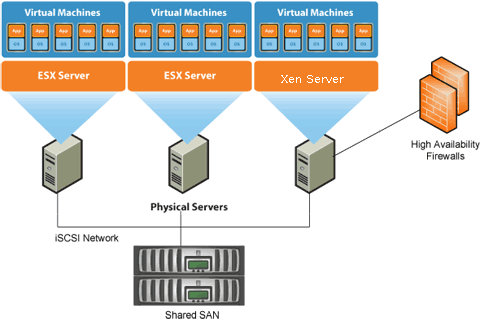
\includegraphics[scale=.4]{imgs/samplecloud.png}
\end{figure}

We define QoS as the performance, the avaibilitity, etc. provided by
a cloud.
Virtualization in clouds allows to
\begin{itemize}
	\item Launch and stop services on the fly
	\item Replicates easily VMs running those services
	\item Facilitate administration
\end{itemize}
\end{frame}

\subsection{Virtualisation and Cloud}
\begin{frame}{Clouds in business}
Large firms delegates their IT infrastructure to specialized companies
\begin{itemize}
	\item Reduction of the costs (less hardware to buy and manage,
		less software to write, etc.)
	\item Augmentation of the QoS
\end{itemize}
However, by doing so, those firms:
\begin{itemize}
	\item Lose control over their data
	\item Become dependent of another company
\end{itemize}
\end{frame}

\begin{frame}{Different types of services}
\begin{figure}[!ht]
	\centering
	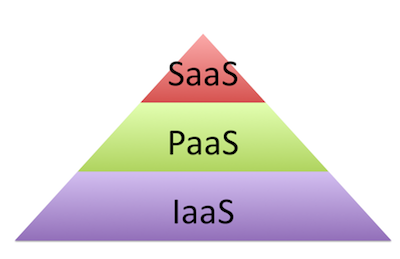
\includegraphics[scale=.45]{imgs/cloud-pyramid.png}
\end{figure}
BtrPlace works at the Infrastructure level.
\end{frame}

\begin{frame}{How is it done?}
There are different kind  of hypervisor,\\
\pause with different features,\\ % follow what the client want
\pause and different licences; % limitations on the ressources usable

Need for a software to manage at the Infrastructure level those
different hypervisors, and provide services such as redundancy of
services.
\end{frame}

\subsection{BtrPlace, a placement manager}
% détails, à supprimer (un item)
\begin{frame}{BtrPlace}
BtrPlace is a software written  by Fabien Hermenier (OASIS team).\\
\pause It aims to solve the problem of distributing a set of VMs on
a set of nodes efficiently, by following some constraints. The latters
can be :
\begin{itemize}
	\item imposed by the hardware, such as available ressources
	\item given by the user, following his needs (eg. replication
		of VMs)
	\item imposed by hypervisors licences
\end{itemize}
\pause As it competitors, BtrPlace doesn't make the distinction
between different hypervisors, but as it was designed to be extensible,
it should be reasonably easy to augment its model to support typing
\end{frame}
\section{Adding typing in BtrPlace}
\subsection{Modelisation in BtrPlace}
\begin{frame}{Modelisation in BtrPlace}
\begin{figure}[!ht]
	\centering
	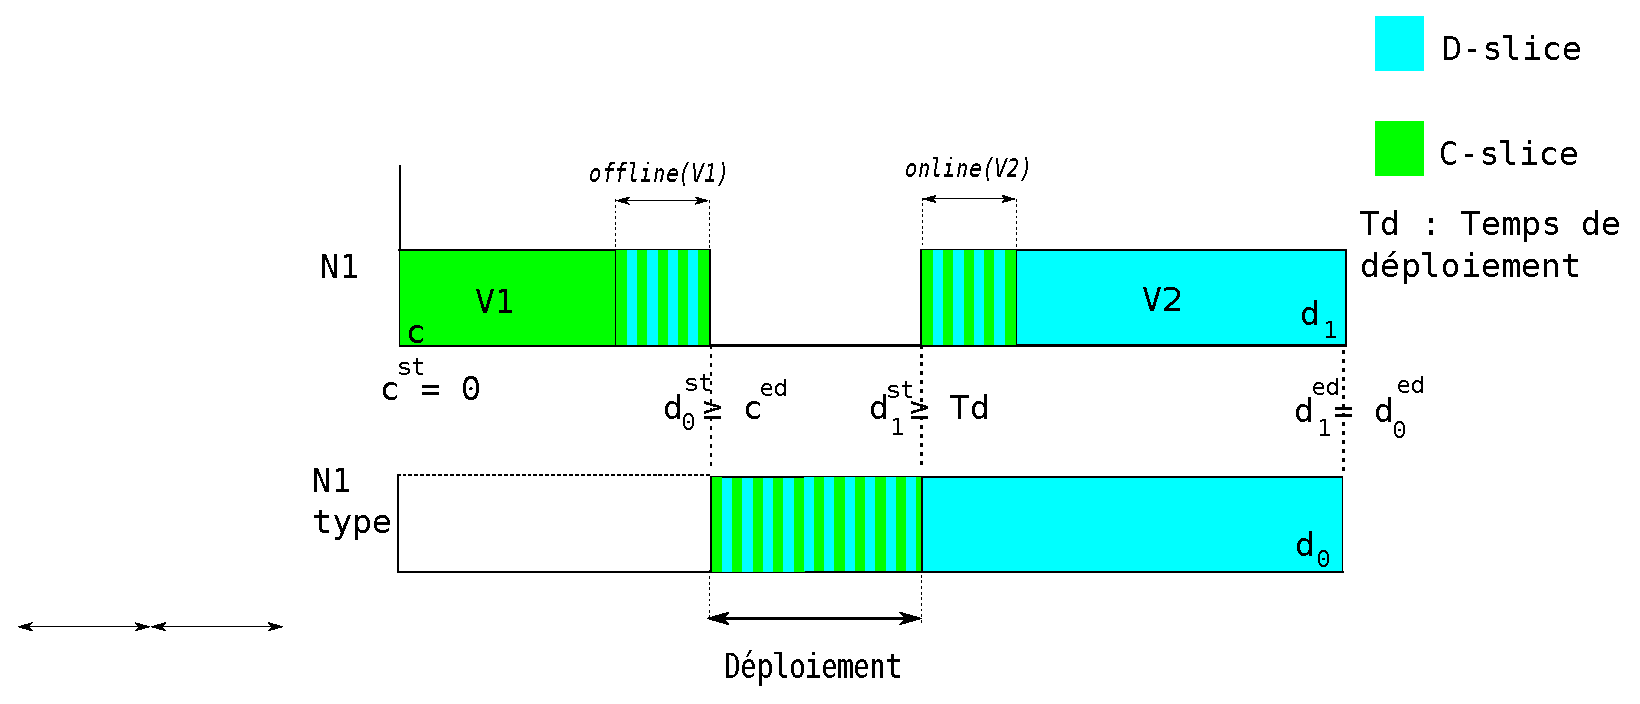
\includegraphics[scale=.4]{imgs/config.eps}
\end{figure}
\begin{itemize}
	\item{\textbf{Type}}, integer associated to each hypervisor
	\item{\textbf{Deployment}}, operation of rebooting a node and
		eventually changing its hypervisor
	\item{\textbf{Reconfiguration}}, operation during which BtrPlace
		change the placement of VMs on nodes following constraints
\end{itemize}
\end{frame}
\begin{frame}{Proceeding of the work}
We worked incrementally by
\begin{enumerate}
	 \item modeling and implementing a special case of the typing
	 \item modeling and implementing the general case
	 \item implementing some constraints associated to typing problems
\end{enumerate}
\end{frame}

\subsection{Special case}
\begin{frame}{Model}
\textbf{Hypothesis}: we know which nodes are going to change their hypervisor,
and the name of the new hypervisor.\\
\pause For such a node, the following constraints must be satisfied:
\[
	P(c) = n \Rightarrow c^\mathrm{ed} \leq D^\mathrm{st}
\]
\[
	P(d) = n \Rightarrow d^\mathrm{st} \geq D^\mathrm{ed}
\]
\pause Placement satisfied iff:
\[
	P(v) = n \Rightarrow T(n) = T(v)	
\]

\end{frame}
\begin{frame}{Code}
This special case is implemented through a constraint
$Platform((n_i, h_j), (n_{i+1}, h_k), \ldots)$.
There are two main methods in this class:
\begin{enumerate}
	\item{\textbf{inject}}, which inject into Choco the two previous
		constraints
	\item{\textbf{isSatisfied}}, which ensures the injected constraints
		are indeed satisfied in the new configuration
\end{enumerate}
\end{frame}

\subsection{General case}
\begin{frame}{Model}
We delete the previous hypothesis : BtrPlace should deduce the new
type of the nodes.\\
We add a vector $v_i$ to each node. $v_i[t]$ represents the number
of VMs running under the hypervisor $t$.
\pause The placement is satisfied iff:
\[
	(\exists ! x \in v_i), x \neq 0
\]

Currently, only the model has been defined correctly, no working code.
\end{frame}

% signature contrainte, schéma + implémenter grace au modèle
\subsection{Additional constraints}
\begin{frame}{MinPlatform}
$MinPlatform(nodes, type, n)$ ensures at least $n$ nodes from $nodes$ runs
hypervisor $type$.
\begin{figure}[!ht]
	\centering
	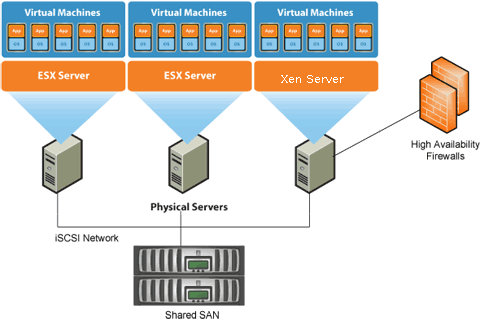
\includegraphics[scale=.4]{imgs/samplecloud.png}
	\caption{Here, BtrPlace could ensure at least two nodes run ESX Server}
\end{figure}
\end{frame}
\begin{frame}{MaxVM}
$MaxVM(nodes, type, n)$ ensures at most $n$ platforms runs of nodes running
hypervisor $type$.\\
\pause Other PFE projects proposed by Fabien in response to licence limitations
(VMWare notably), easily implemented because typing is done with integer.
\end{frame}

\section{Management}
\subsection{Problems encountered}
\begin{frame}{Timing management}
\begin{figure}[!ht]
	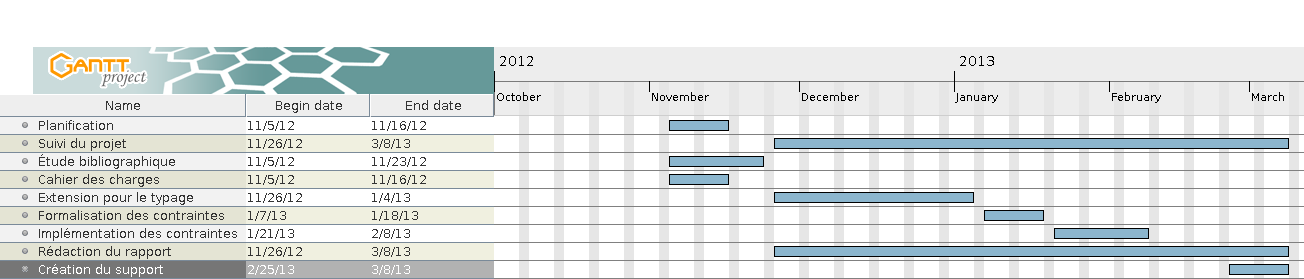
\includegraphics[scale=.2]{imgs/gantt2.png}
\end{figure}
\textbf{Problem}: not enough time spent on timing the work; incoherence
in the DOW observed at the end of the project, leading to badly structured
reports.\\
\pause\textbf{Possible Solution} : spend more time on timing and structuring the
work rather than on writing others parts of the DOW. Try to evaluate better
exogenous elements (mainly other scholar works).
\end{frame}

\begin{frame}{Complexity of BtrPlace}
\textbf{Problem} : only documentation available : API Java.
Inadequate and insufficient to understand fully BtrPlace.\\
\pause\textbf{Possible solution} : add two more layers of documentation.
\begin{enumerate}
	\item one describing the general structure of the software, with
		some example
	\item one more precise than the latter, containing information about
		model generation and how to write simple constraints
\end{enumerate}
\end{frame}

\subsection{Incomplete work}
\begin{frame}{What's done and what's missing?}
\begin{center}
\begin{scriptsize}
\begin{tabular}{c|c}
	\textbf{Goals} & \textbf{State}\\
	\hline
	\hline
	Modelisation of the special case & done \\
	\hline
	Implementation of the special case & partial (insufficient testing) \\
	\hline
	Modelisation of the general case & done \\
	\hline
	Implementation of the general case & partial (not at the right place) \\
	\hline
	Modelisation of new constraints & not done (easy and fast to do) \\
	\hline
	Implementation of new constraints & mostly done (lack of printer/getters, testing) \\
	\hline
\end{tabular}
\end{scriptsize}
\end{center}
\end{frame}

\section{To sum up}
\begin{frame}{New competences and technologies}
During this project, I learnt and revisited:
\begin{itemize}
	\item Java and related tools (maven, IntelliJ, unit testing)
	\item Management of ressources and combinatorial problems
	\item Choco framework
	\item Git
\end{itemize}
\end{frame}
\begin{frame}{How to improve what has been done}
To be complete, one may add a few more test for the special case.\\
\pause The general case, should be implemented at the right place, and not
as a user constraint, and tested correctly.\\
\pause Models for the constraints \textit{MinPlatform} and \textit{MaxVM}
should be defined, and implementations revisited following the established
models. 
\end{frame}
\begin{frame}{Possible evolutions thanks to typing}
Hypervisors licences and features can be pretty differents:
\begin{itemize}
	\item some allows migrating VMs, some don't
	\item some put restrictions on usable hardware (number of NIC, RAM, CPU usable
		by the hypervisor)
	\item etc.
\end{itemize}
Typing could help modelize those limitations.
\end{frame}

\begin{frame}{Questions}
\begin{center}
Thanks for your attention and time. Do you have any questions?
\end{center}
\end{frame}

% à envoyer, plus copie fh
\end{document}